\documentclass{article}
\usepackage[utf8]{inputenc}

\title{Diseño de la base de datos}
\author{Alejandro Iabin Arteaga Hernández}
\date{Diciembre 2019}

\usepackage{natbib}
\usepackage{graphicx}

\begin{document}

\maketitle

\section{Modelo Entidad - Relación}

\begin{figure}[h!]
\centering
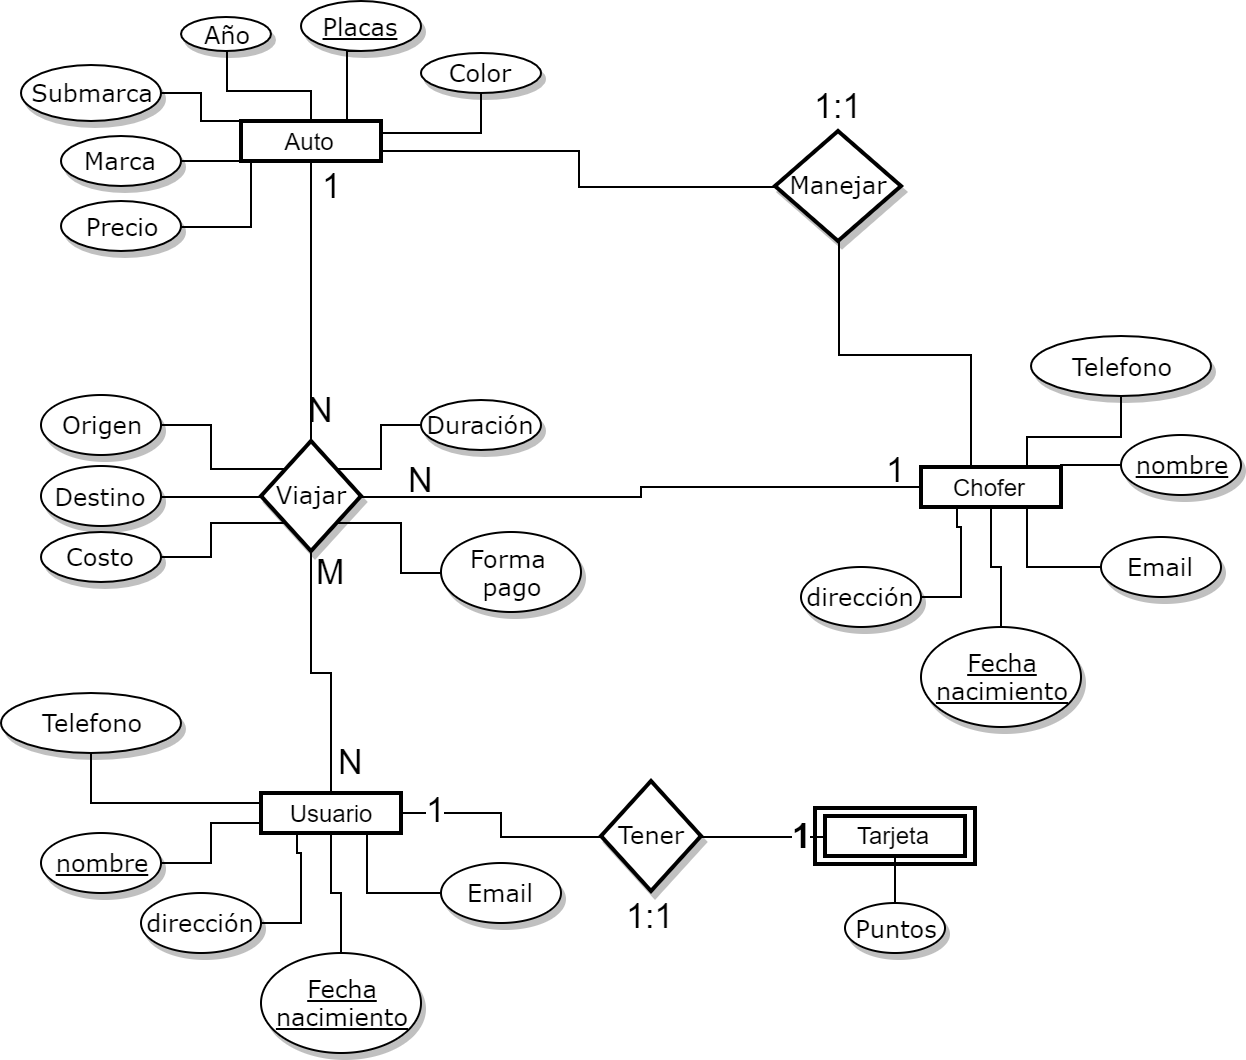
\includegraphics[scale=0.32]{er.png}
\caption{Modelo Entidad - Relación}
\end{figure}
\newpage
\subsection{Justificación de las relaciones}
Cada usuario tiene una tarjeta digital y cada tarjeta digital tiene asignado un único usuario, esa es la razón por la cual la relación \textbf{Tener} es una relación uno a uno. \par\null\par
\textbf{Tarjeta} al no tener llave candidata, y depender de la entidad \textbf{Usuario} es una entidad débil.
\par\null\par
Respecto a la relación \textbf{Viajar}, es una relación terciaria, además de ser muy importante para los requerimientos de la aplicación, ya que es la relación que mantiene el caso de uso principal del la aplicación, la cual es gestionar viajes, es una relación N:M  ya que: varios usuarios pueden tomar varios viajes (Compartido), pero es N:1 con Chofer y Auto debido a que estos viajes solo puede tener un \textbf{Auto} y un \textbf{Chofer}.\par\null\par
Y acerca de la relación \textbf{Manejar}, es importante ponerla ya que satisface el caso de uso de que los choferes deben saber que coche les toca y que vayan rotando cada semana.
\par\null\par
Y acerca de las llaves candidatas en el modelo Entidad - relación,
se escogió \textbf{Placa} para la tabla auto, ya que es un atributo único de cada auto, de igual manera que la tupla (nombre, fechaNacimiento) para la entidad Usuario y la entidad Chofer
\newpage
\section{Modelo Relacional}
\begin{figure}[h!]
\centering
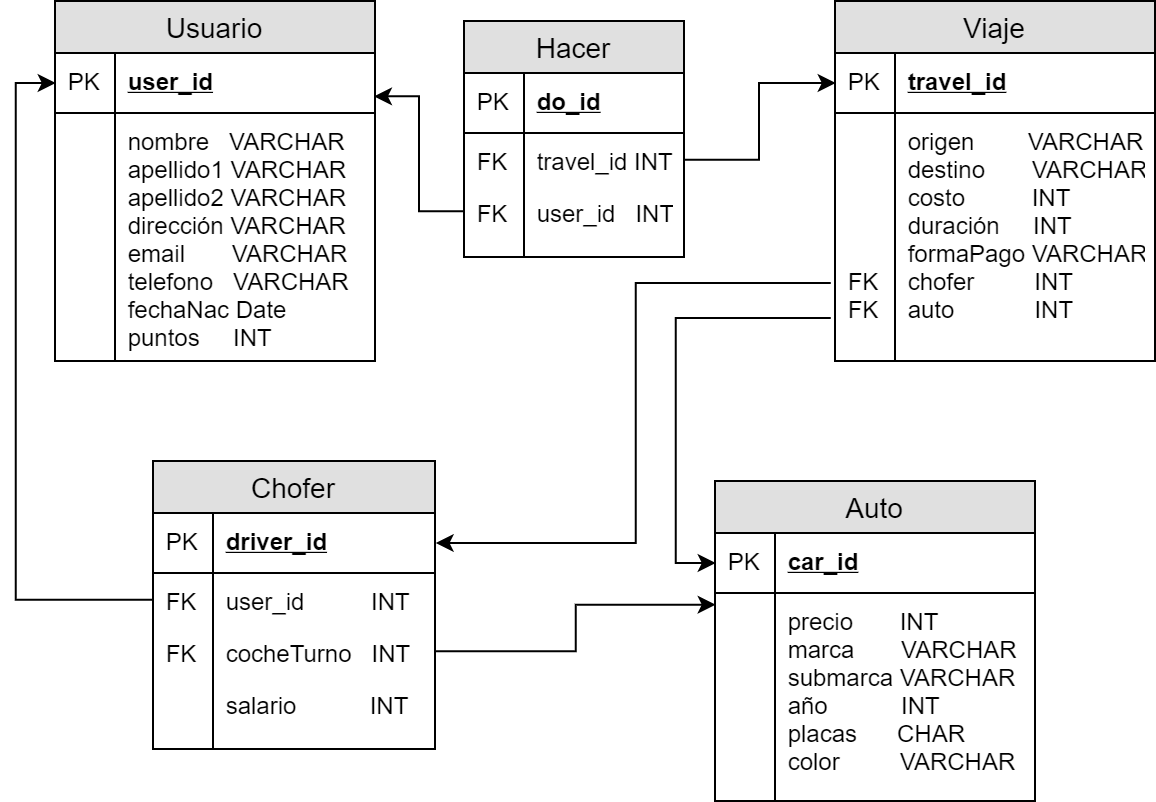
\includegraphics[scale=0.32]{relacional.png}
\caption{Modelo relacional}
\end{figure}
\newpage
\subsection{Modelo relacional, justificación}
El primer paso para traducir el modelo, fue traducir las entidades más fáciles de identificar, ya que tienen traducción directa en tablas, fueron \textbf{Usuario y Auto}, lo primero fue decidir cual sería la llave primaria.\par\null\par
Decidí poner una llave artificial, insertada por decisión de diseño: los \textbf{\textit{id}}, esa será la llave de cada una de las tablas, debido a que las consultas funcionan más eficientemente y esos ids artificiales no dependen funcionalmente de ningún otro atributo o factor externo, por ejemplo si usamos la placa como llave primaria, esta podría cambiar en el tiempo y sería problemático para la integridad de nuestros datos, además de que si se les pone un id que va incrementándose, podemos tener nuestra tabla ordenada por tiempo, sin necesidad de almacenar la fecha. Por ello creo que es beneficioso agregar un id autoincrementable a cada tabla.
\par\null\par
Después de eso, fue agregar los campos de cada tabla, el primer paso fue agregar el atributo multivaluado nombre como los 3 atributos que en realidad es, nombre, apellido paterno y materno. De igual manera, al ser una relación 1 a 1, agregué el atributo de los puntos de la tarjeta a cada usuario, otro de los atributos que pueden ser multivaluados son teléfono e email. Por el momento no nos ocuparemos de ellos, pero en la normalización se hará una tabla nueva para ellos.\par\null\par
Viajar al ser una relación que incluye mucho, se generó una tabla nueva que contiene los atributos de la relación, respecto a las relaciones con las otras tablas, con usuario al ser muchos a muchos, se tuvo que hacer una tabla de unión, que almacenara los usuarios que tomaron cierto viaje, y como las relaciones con auto y chofer son 1 a 1, se agregó una llave foránea que hace referencia a las llaves primarias de Auto y Chofer\par\null\par
El último reto de la traducción a modelo relacional fue la tabla Chofer, debido a que Chofer tiene los mismo atributos que la tabla usuario, para evitar redundancias de información, los datos del chofer se guardarán en la tabla usuarios, y la tabla chofer solo tendrá una referencia a su usuario en forma de llave foranea, solo se agregarán los datos extras necesarios, como fue el salario y el auto que le toca manejar el cual es una llave foránea que hace referencia a un Auto.



\end{document}
